\documentclass[a4paper,12pt]{article}
%%%%%%%%%%%%%%%%%%%%%%%%%%%%%%%%%%%%%%%%%%%%%%%%%%%%%%%%%%%%%%%%%%%%%%%%%%%%%%%%%%%%%%%%%%%%%%%%%%%%%%%%%%%%%%%%%%%%%%%%%%%%%%%%%%%%%%%%%%%%%%%%%%%%%%%%%%%%%%%%%%%%%%%%%%%%%%%%%%%%%%%%%%%%%%%%%%%%%%%%%%%%%%%%%%%%%%%%%%%%%%%%%%%%%%%%%%%%%%%%%%%%%%%%%%%%
\usepackage{eurosym}
\usepackage{vmargin}
\usepackage{amsmath}
\usepackage{graphics}
\usepackage{epsfig}
\usepackage{subfigure}
\usepackage{fancyhdr}

\setcounter{MaxMatrixCols}{10}
%TCIDATA{OutputFilter=LATEX.DLL}
%TCIDATA{Version=5.00.0.2570}
%TCIDATA{<META NAME="SaveForMode"CONTENT="1">}
%TCIDATA{LastRevised=Wednesday, February 23, 201113:24:34}
%TCIDATA{<META NAME="GraphicsSave" CONTENT="32">}
%TCIDATA{Language=American English}

\pagestyle{fancy}
\setmarginsrb{20mm}{0mm}{20mm}{25mm}{12mm}{11mm}{0mm}{11mm}
\lhead{MA4128} \rhead{Kevin O'Brien} \chead{Week 6} %\input{tcilatex}

\begin{document}

\tableofcontents
\newpage

% http://www.norusis.com/pdf/SPC_v13.pdf
\section{Agenda for Today's Class}

\begin{itemize}
\item Review of Important Topics
\item Review of K-Means Clustering (SPSS Exercise)
\item Two-Step Clustering
\item Review of Regression (Optional for Math Science Students)
\end{itemize}

\section{Important Topics}

\begin{itemize}
\item \textbf{Multi-collinearity}: Multi-collinearity occurs when two or more predictors in the model are
correlated and provide redundant information about the response. Examples of pairs of multi-collinear predictors are years of education and income, height and weight of a person, and assessed value and square footage
of a house.

\item \textbf{Consequences of high multicollinearity}:
Multi-collinearity leads to decreased reliability and predictive power of statistical models, and hence, very often, confusing and misleading results.
\item Multicollinearity will be dealt with in a future component of this course: Variable Selection Procedures.
\end{itemize}

%------------------------------------------------------------------%
\newpage
\section{Two-Step Cluster Analysis}

When you have a really large data set or you need a clustering procedure that can rapidly form clusters on the basis of either categorical or continuous data, neither of the previous two procedures are entirely appropriate. Hierarchical clustering requires a matrix of distances between all pairs of cases, and k-means requires shuffling cases in and out of clusters and knowing the number of clusters in advance.

The Two-Step Cluster Analysis procedure was designed for such applications. The name two-step clustering is already an indication that the algorithm is based on a two-stage approach
\begin{itemize}
\item In the first stage, the algorithm undertakes a procedure that is very similar to the k-means algorithm. \item Based on these results, the two-step
procedure conducts a modified hierarchical agglomerative clustering procedure that
combines the objects sequentially to form homogenous clusters.
\end{itemize}

The Two-Step Cluster Analysis is an exploratory tool designed to reveal natural groupings (or clusters) within a data set that would otherwise not be apparent. The algorithm employed by this procedure has several desirable features that differentiate it from traditional clustering techniques:

\begin{itemize}
\item Handling of categorical and continuous variables. By assuming variables to be independent, a joint \textbf{\textit{multinomial-normal distribution}} can be placed on categorical and continuous variables. (Interesting, but not examinable).

 \item Automatic selection of number of clusters. By comparing the values of a \textbf{\textit{model-choice criterion}} across different clustering solutions, the procedure can automatically determine the optimal number of clusters.

\item Scalability. By constructing a \textbf{\textit{cluster features}} (CF) tree that summarizes the records, the Two-Step algorithm allows you to analyze large data files. The Two-Step Cluster Analysis requires only one pass of data (which is important for very large data files).

\end{itemize}


%-----------------------------------------------------------------------------%
\newpage
\subsection{Pre-clustering }

In two-step clustering, to make large problems tractable, in the first step, cases are
assigned to \textbf{\textit{preclusters}}. In the second step, the preclusters are clustered using the
hierarchical clustering algorithm. You can specify the number of clusters you want or
let the algorithm decide based on preselected criteria.

In general, the larger the number of sub-clusters produced by the pre-cluster step, the more accurate the final result is. However, too many sub-clusters will slow down the clustering during the second step.

The maximum number of sub-clusters should be carefully chosen so that it is large enough to produce accurate results and small enough not to slow down the second step clustering.




\subsubsection{Step 1: Preclustering: Making Little Clusters}
The first step of the two-step procedure is formation of preclusters. The goal of
preclustering is to reduce the size of the matrix that contains distances between all
possible pairs of cases. Preclusters are just clusters of the original cases that are used
in place of the raw data in the hierarchical clustering. As a case is read, the algorithm
decides, based on a distance measure, if the current case should be merged with a
previously formed precluster or start a new precluster. When preclustering is complete,
all cases in the same precluster are treated as a single entity. The size of the distance
matrix is no longer dependent on the number of cases but on the number of preclusters.

\subsubsection{Step 2: Hierarchical Clustering of Preclusters}
In the second step, SPSS uses the standard hierarchical clustering algorithm on the
preclusters. Forming clusters hierarchically lets you explore a range of solutions with
different numbers of clusters.


%----------------------------------------------------------------------%
\section{Important Considerations for Two-Step Clustering}
\subsection{Cluster Features Tree}

Two-Step Cluster Analysis is done by building a so-called \textbf{\textit{cluster feature tree}} whose \textbf{\textit{leaves}} represent distinct objects in the dataset. The procedure can handle categorical and continuous variables simultaneously and offers the user the flexibility to specify the cluster numbers as well as the maximum number of clusters, or to allow the technique to automatically choose the number of clusters on the basis of statistical evaluation criteria.

Additionally, the procedure indicates each variable�s importance for the construction of a specific cluster. These desirable features make the somewhat less popular two-step clustering a viable alternative to the traditional
methods.


\subsection{Types of Data} The Two-Step procedure works with both continuous and categorical variables. Cases represent objects to be clustered, and the variables represent attributes upon which the clustering is based.

\subsection{Case Order}
Note that the cluster features tree and the final solution may depend on the order of objects (or cases). To minimize order effects, randomly order the cases. It is recommended to obtain several different solutions with cases sorted in different random orders to verify the stability of a given solution. In situations where this is difficult due to extremely large file sizes, multiple runs with a sample of cases sorted in different random orders might be substituted.
%------------------------------------------------------------------------------%
\newpage
\section{SPSS Implementation}

\begin{itemize}
\item To implement a Two-Step Cluster Analysis in SPSS, you use the following options:\\
\textbf{\textit{Analyze $>$ Classify $>$ TwoStep Cluster}}.

\item \textbf{Distance Measure} Log likelihood distance measures are the default; Euclidean distance can be used if all variables are continuous. (Log likelihood distance measures are not part of course).

\item \textbf{Count of Continuous Variables} Continuous variables are standardized by default. The variables
are standardized so that they all contribute equally to the distance or similarity between cases.

\item \textbf{Number of clusters} You can specify the number of clusters, or you can let the algorithm select
the optimal number based on either the Schwarz Bayesian criterion (BIC) or the Akaike
information criterion (AIC).

\item \textbf{Clustering Criterion} BIC and AIC are offered with the default being BIC.
\end{itemize}


\subsection{Graphical Outputs}
The lower part of the output  indicates the quality of the cluster
solution. The silhouette measure of cohesion and separation is a measure of the
clustering solution�s overall goodness-of-fit. It is essentially based on the average
distances between the objects and can vary between -1 and +1. Specifically, a
silhouette measure of less than 0.20 indicates a poor solution quality, a measure
between 0.20 and 0.50 a fair solution, whereas values of more than 0.50 indicate a
good solution . In our case, the measure indicates a satisfactory (``fair") cluster quality. Consequently, you can
proceed with the analysis by double-clicking on the output. This will open up the
model viewer , an evaluation tool that graphically presents the structure
of the revealed clusters.


The model viewer provides us with two windows: the main view, which initially
shows a model summary (left-hand side), and an auxiliary view, which initially
features the cluster sizes (right-hand side). At the bottom of each window, you can
request different information, such as an overview of the cluster structure and the
overall variable importance.
%------------------------------------------------------------------------------%
\newpage

\section{ More on Two-Step Clustering}
\subsection{Step 1: Pre-clustering: Making Little Clusters}
The first step of the two-step procedure is formation of pre-clusters. The goal of pre-clustering is to reduce the size of the Distance matrix (the matrix that contains distances between all
possible pairs of cases). Pre-clusters are just clusters of the original cases that are used in place of the raw data in the hierarchical clustering. As a case is read, the algorithm
decides, based on a distance measure, if the current case should be merged with a previously formed pre-cluster or start a new precluster.

When preclustering is complete, all cases in the same precluster are treated as a single entity. The size of the distance matrix is no longer dependent on the number of cases but on the number of preclusters.

\subsection{Step 2: Hierarchical Clustering of Preclusters}
In the second step, SPSS uses the standard hierarchical clustering algorithm on the
preclusters. Forming clusters hierarchically lets you explore a range of solutions with
different numbers of clusters.
Tip: The Options dialog box lets you control the number of preclusters. Large numbers
of preclusters give better results because the cases are more similar in a precluster;
however, forming many preclusters slows the algorithm.

%-------------------------------------------------------------------------%
\newpage
\section{Examining the Number of Clusters}


\newpage

\section{Linear Regression Analysis}

\subsection{Introduction}
Linear regression is used when you want to predict the value of a variable based on the value of another variable. The variable we want to predict is called the dependent variable (or sometimes, the outcome variable). The variable we are using to predict the other variable's value is called the independent variable (or sometimes, the predictor variable).


For example, you could use linear regression to understand whether exam performance can be predicted based on revision time; whether cigarette consumptions can be predicted based on smoking duration; and so forth. If you have two or more independent variables, rather than just one, you need to use \textbf{\textit{multiple regression}}.

SPSS can be used to carry out linear regression, as well as interpret and report the results from this test. However, before we introduce you to this procedure, you need to understand the different assumptions that your data must meet in order for linear regression to give you a valid result. We discuss these assumptions next.


\subsection{Assumptions}
When you choose to analyse your data using linear regression, part of the process involves checking to make sure that the data you want to analyse can actually be analysed using linear regression. You need to do this because it is only appropriate to use linear regression if your data is appropriate for six assumptions that are required for linear regression to give you a valid result.

In practice, checking for these six assumptions just adds a little bit more time to your analysis, requiring you to click a few more buttons in SPSS when performing your analysis, as well as think a little bit more about your data, but it is not a difficult task.

Often when analysing your own data using SPSS, one or more of these assumptions is violated (i.e., not met). This is not uncommon when working with real-world data rather than textbook examples, which often only show you how to carry out linear regression when everything goes well. However, even when your data fails certain assumptions, there is often a solution to overcome this. First, let�s take a look at these six assumptions:

\begin{itemize}
\item \textbf{Assumption 1}: Your two variables should be measured at the interval or ratio level (i.e., they are continuous). Examples of variables that meet this criterion include revision time (measured in hours), intelligence (measured using IQ score), exam performance (measured from 0 to 100), weight (measured in kg), and so forth. You can learn more about interval and ratio variables in our article: Types of Variable.

\item \textbf{Assumption 2}: There needs to be a linear relationship between the two variables. Whilst there are a number of ways to check whether a linear relationship exists between your two variables, we suggest creating a scatter-plot using SPSS, where you can plot the dependent variable against your independent variable, and then visually inspect the scatter-plot to check for linearity. Your scatter-plot may look something like one of the following:

If the relationship displayed in your scatterplot is not linear, you will have to either run a non-linear regression analysis or \textbf{\textit{transform}} your data, which you can do using SPSS. It is important to learn how to: (a) create a scatterplot to check for linearity when carrying out linear regression using SPSS; (b) interpret different scatterplot results; and (c) transform your data using SPSS if there is not a linear relationship between your two variables.

\begin{figure}[h!]
\begin{centering}
  % Requires \usepackage{graphicx}
  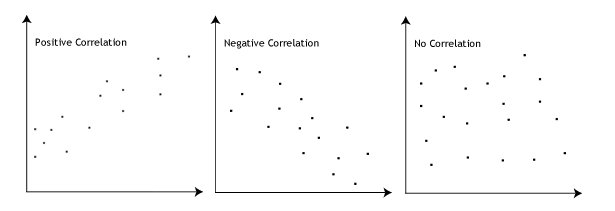
\includegraphics[width=10cm]{Regre1.jpg}\\
  \caption{Types of Linear Relationship}
\end{centering}
\end{figure}

\item \textbf{Assumption 3}: There should be no significant outliers. Outliers are simply single data points within your data that do not follow the usual pattern (e.g., in a study of 100 students� IQ scores, where the mean score was 108 with only a small variation between students, one student had a score of 156, which is very unusual, and may even put her in the top 1\% of IQ scores globally). The following scatterplots highlight the potential impact of outliers:

The problem with outliers is that they can have a negative effect on the regression equation that is used to predict the value of the dependent (outcome) variable based on the independent (predictor) variable. This will change the output that SPSS produces and reduce the predictive accuracy of your results. Fortunately, when using SPSS to run linear regression on your data, you can easily include criteria to help you detect possible outliers.
\begin{figure}[h!]
\begin{centering}
  % Requires \usepackage{graphicx}
  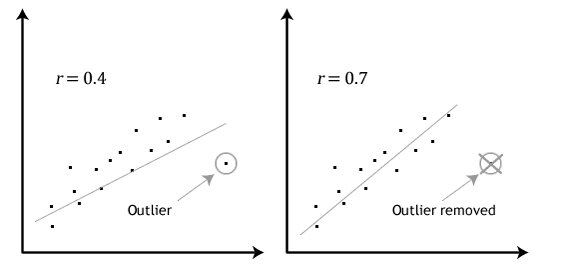
\includegraphics[width=10cm]{Regre2.jpg}\\
  \caption{Effect of an Outlier}
\end{centering}
\end{figure}
%In our enhanced linear regression guide, we: (a) show you how to detect outliers using \textbf{case-wise diagnostics}, which is a simple process when using SPSS; and (b) discuss some of the options you have in order to deal with outliers.
\item \textbf{Assumption 4}: You should have independence of observations, which you can easily check using the Durbin-Watson statistic, which is a simple test to run using SPSS. We explain how to interpret the result of the Durbin-Watson statistic later.

\item \textbf{Assumption 5}:Your data needs to show \textbf{\textit{homoscedasticity}}, which is where the variances along the line of best fit remain similar as you move along the line. Whilst we explain more about what this means and how to assess the homoscedasticity of your data in the linear regression line, take a look at the two scatter-plots below, which provide two simple examples: one of data that meets this assumption and one that fails the assumption:

\begin{figure}[h!]
\begin{centering}
  % Requires \usepackage{graphicx}
  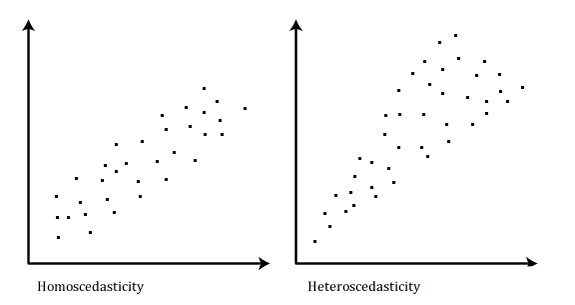
\includegraphics[width=10cm]{Regre3.jpg}\\
  \caption{Constant Variance}
\end{centering}
\end{figure}
When you analyse your own data, you will be lucky if your scatterplot looks like either of the two above. Whilst these help to illustrate the differences in data that meets or violates the assumption of homoscedasticity, real-world data is often a lot more messy. Therefore, in our enhanced linear regression guide, we explain: (a) some of the things you will need to consider when interpreting your data; and (b) possible ways to continue with your analysis if your data fails to meet this assumption.
\item \textbf{Assumption 6}:Finally, you need to check that the residuals (errors) of your two variables are approximately normally distributed (we explain these terms in our enhanced linear regression guide). Two common methods to check this assumption include using either a histogram (with a superimposed normal curve) or by using a Normal P-P Plot.
  %  Again, in our enhanced linear regression guide, we: (a) show you how to check this assumption using SPSS, whether you use a histogram (with superimposed normal curve) or Normal P-P Plot; (b) explain how to interpret these diagrams; and (c) provide a possible solution if your data fails to meet this assumption.

\end{itemize}
You can check assumptions all assumptions except no.1 using SPSS. It is recommended to test these assumptions in this order because it represents an order where, if a violation to the assumption is not correctable, you will no longer be able to use a single linear regression (although you may be able to run another statistical test on your data instead). Just remember that if you do not run the statistical tests on these assumptions correctly, the results you get when running a linear regression might not be valid.


\end{document}
%------------------------------------------------------------------------------%\end{document}


